\section{Related Work}

\subsection{LLMs as Financial Assistants}

Large Language Models (LLMs) are applied in finance by fine-tuning on financial data or training on financial corpora. This improves the model’s understanding of financial terminology and data, enabling a specialized assistant for analytical support, insights, and information retrieval, rather than trade execution. 


\textbf{Fine-Tuned LLMs for Finance}

Fine-tuning enhances domain-specific performance. Examples include PIXIU (FinMA) \citep{xie2023pixiu}, which fine-tuned LLaMA on 136K finance-related instructions; FinGPT \citep{touvron2023llama2openfoundation, yang2023fingpt}, which used LoRA to fine-tune models like LLaMA and ChatGLM with about 50K finance-specific samples; and Instruct-FinGPT \citep{zhang2023instructfingpt}, fine-tuned on 10K instruction samples from financial sentiment analysis datasets. These models outperform their base versions and other open-source LLMs like BLOOM and OPT \citep{zhang2022opt} in finance classification tasks, even surpassing BloombergGPT \citep{wu2023bloomberggpt} in several evaluations. However, in generative tasks, they perform similarly or slightly worse than powerful general-purpose models like GPT-4, indicating a need for more high-quality, domain-specific datasets.

\textbf{Finance LLMs Trained from Scratch}

Training LLMs from scratch on finance-specific corpora aims for better domain adaptation. Models like BloombergGPT \citep{wu2023bloomberggpt}, XuanYuan 2.0 \citep{zhang2023xuanyuan}, and Fin-T5 \citep{lu2023bbtfin} combine public datasets with finance-specific data during pretraining. BloombergGPT, for instance, was trained on both general and financial text, with proprietary Bloomberg data enhancing its performance on finance benchmarks. These models outperform general-purpose counterparts like BLOOM-176B and T5 in tasks such as market sentiment classification and summarization. While they may not match larger closed-source models like GPT-3 or PaLM \citep{chowdhery2022palm}, they offer competitive performance among similar-sized open-source models without compromising general language understanding.

In summary, finance-specific LLMs developed through fine-tuning or training from scratch show significant improvements in domain-specific tasks, underscoring the importance of domain adaptation and the potential for further enhancements with high-quality finance-specific datasets.

\begin{figure*}[htbp]
\centerline{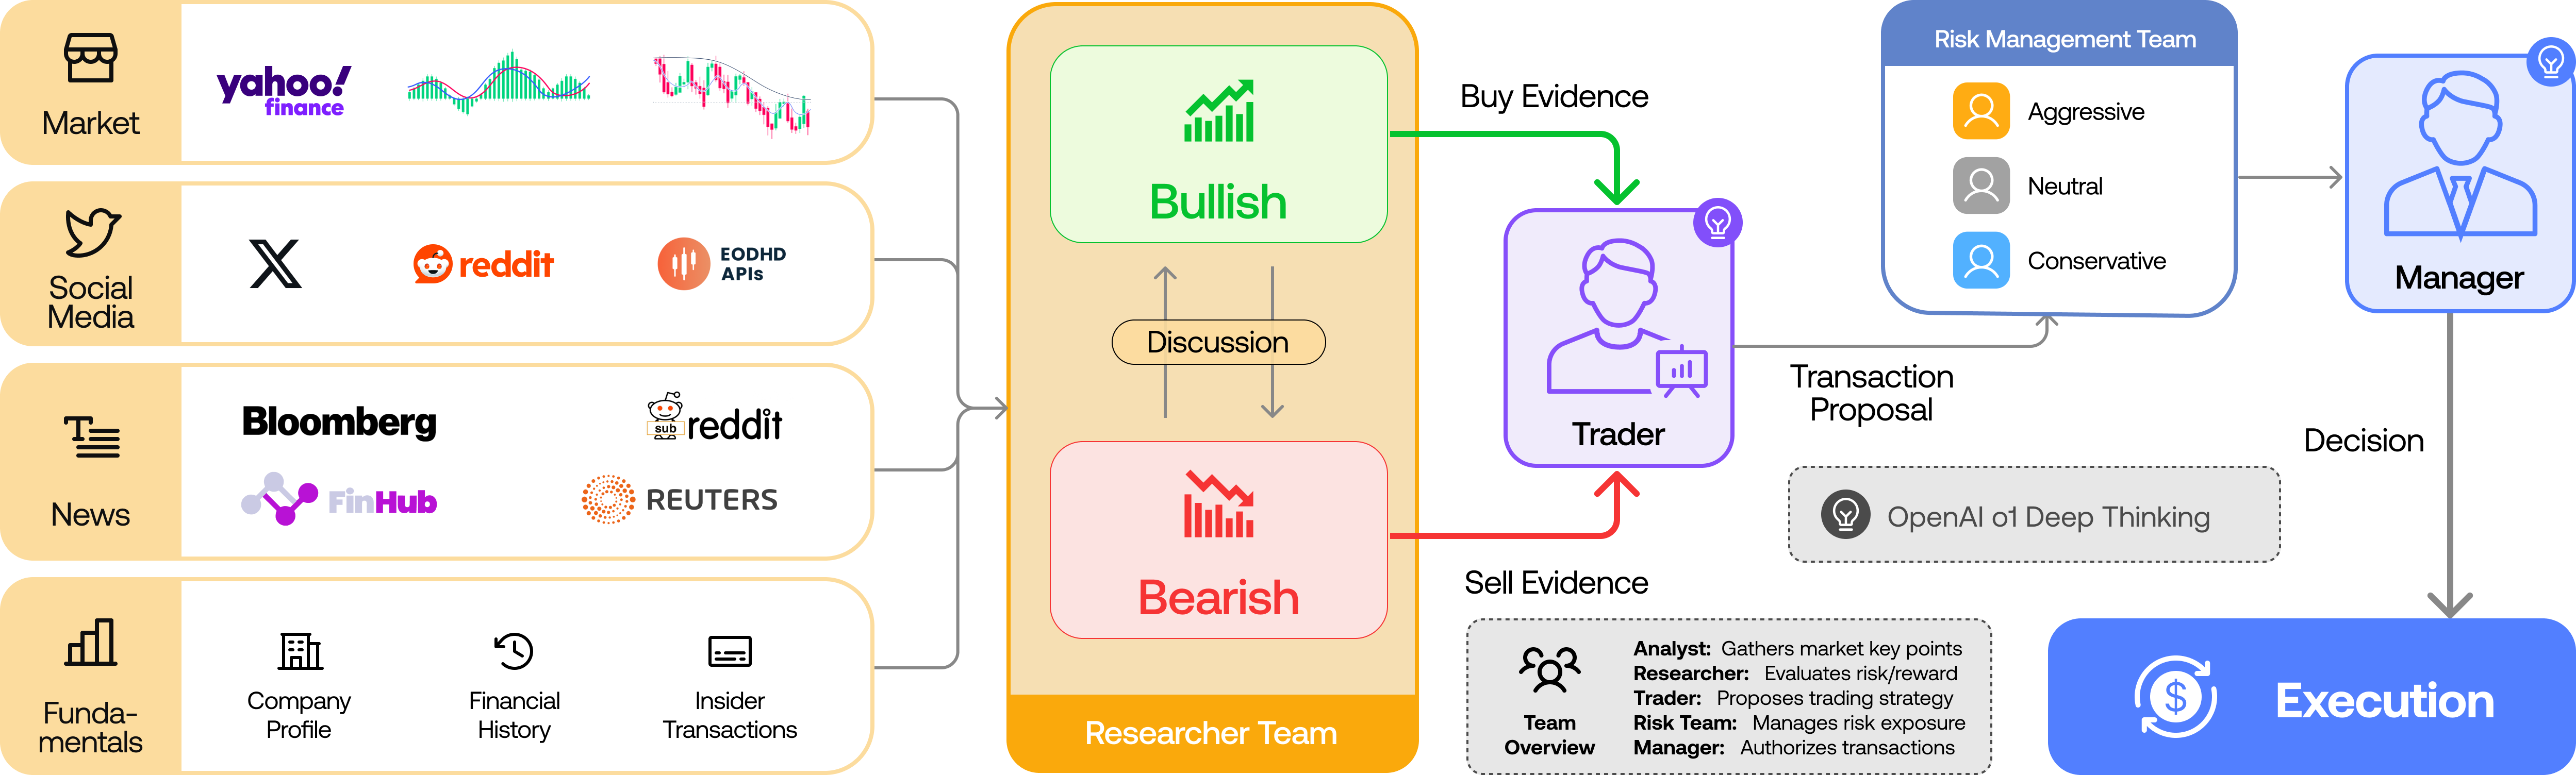
\includegraphics[width=\linewidth]{figures/schema.png}}
\caption{\textbf{\textcolor{brown}{\model}} Overall Framework Organization. \textsc{\textbf{I. Analysts Team}}: Four analysts concurrently gather relevant market information. \textsc{\textbf{II. Research Team}}: The team discusses and evaluates the collected data. \textsc{\textbf{III. Trader}}: Based on the researchers' analysis, the trader makes the trading decision. \textsc{\textbf{IV. Risk Management Team}}: Risk guardians assess the decision against current market conditions to mitigate risks. \textsc{\textbf{V. Fund Manager}}: The fund manager approves and executes the trade.}
\label{schema}
\end{figure*}



\subsection{LLMs as Traders}

LLMs act as trader agents making direct trading decisions by analyzing external data like news, financial reports, and stock prices. Proposed architectures include news-driven, reasoning-driven, and reinforcement learning (RL)-driven agents.

\textbf{News-Driven Agents}

News-driven architectures integrate stock news and macroeconomic updates into LLM prompts to predict stock price movements. Studies evaluating both closed-source models (e.g., GPT-3.5, GPT-4) and open-source LLMs (e.g., Qwen \citep{bai2023qwentechnicalreport}, Baichuan \citep{yang2023baichuan2openlargescale}) in financial sentiment analysis have shown the effectiveness of simple long-short strategies based on sentiment scores \citep{lopezlira2023chatgptforecaststockprice}. Further research on fine-tuned LLMs like FinGPT and OPT demonstrates improved performance through domain-specific alignment \citep{unveiling, sentitrade}. Advanced methods involve summarizing news data and reasoning about their relationship with stock prices \citep{beatunveiling, wang2024llmfactorextractingprofitablefactors}.

\textbf{Reasoning-Driven Agents}

Reasoning-driven agents enhance trading decisions through mechanisms like reflection and debate. Reflection-driven agents, such as FinMem \citep{finmem} and FinAgent \citep{multimodalfinmem}, use layered memorization and multimodal data to summarize inputs into memories, inform decisions, and incorporate technical indicators, achieving superior backtest performance while mitigating hallucinations \citep{ji2023mitigatinghallucinationlargelanguage}. Debate-driven agents, like those in heterogeneous frameworks \citep{xing2024designingheterogeneousllmagents} and TradingGPT \citep{li2023tradinggptmultiagentlayeredmemory}, enhance reasoning and factual validity by employing LLM debates among agents with different roles, improving sentiment classification and increasing robustness in trading decisions.

\textbf{Reinforcement Learning-Driven Agents}

Reinforcement learning methods align LLM outputs with expected behaviors, using backtesting as rewards. SEP \citep{Koa_2024} employs RL with memorization and reflection to refine LLM predictions based on market history. Classical RL methods are also used in trading frameworks that integrate LLM-generated embeddings with stock features, trained via algorithms like Proximal Policy Optimization (PPO) \citep{ding2023integratingstockfeaturesglobal, ppo}.

\subsection{LLMs as Alpha Miners}

LLMs are also used to generate alpha factors instead of making direct trading decisions. QuantAgent \citep{wang2023alpha} demonstrates this by leveraging LLMs to produce alpha factors through an inner-loop and outer-loop architecture. In the inner loop, a writer agent generates a script from a trader's idea, while a judge agent provides feedback. In the outer loop, the code is tested in the real market, and trading results enhance the judge agent. This approach enables progressive approximation of optimal behavior.

Subsequent research, such as AlphaGPT \citep{wang2023alpha}, proposes a human-in-the-loop framework for alpha mining with a similar architecture. Both studies showcase the effectiveness of LLM-powered alpha mining systems, highlighting their potential in automating and accelerating the development of trading strategies by generating and refining alpha factors.
